% hmmm... ...you need to supply your own "figma.pdf"...
% that is 1 page cover file, i removed it for my own privacie (⁠ᗒ⁠ᗩ⁠ᗕ⁠)
\documentclass{article}
\usepackage{listings}
\usepackage{xcolor}
\usepackage{indentfirst}
\usepackage{pdfpages}
\usepackage[tmargin=2cm, bmargin=2cm, lmargin=3cm, rmargin=3cm, a4paper]{geometry}

% New colors defined below
\definecolor{codegreen}{rgb}{0,0.6,0}
\definecolor{codegray}{rgb}{0.5,0.5,0.5}
\definecolor{codepurple}{rgb}{0.58,0,0.82}
\definecolor{backcolour}{rgb}{0.95,0.95,0.92}

% di-ubah oleh Antonomasia, dari inisial F
\definecolor{outputbackcolour}{rgb}{0,0,0} % Warna background hitam untuk output
\definecolor{outputcodecolor}{rgb}{1,1,1}  % Warna tulisan putih untuk output

% Code listing style named "mystyle"
\lstdefinestyle{mystyle}{
  backgroundcolor=\color{backcolour},   commentstyle=\color{codegreen},
  keywordstyle=\color{magenta},
  numberstyle=\tiny\color{codegray},
  stringstyle=\color{codepurple},
  basicstyle=\ttfamily\footnotesize,
  breakatwhitespace=false,         
  breaklines=true,                 
  captionpos=b,                    
  keepspaces=true,                 
  numbers=left,                    
  numbersep=5pt,                  
  showspaces=false,                
  showstringspaces=false,
  showtabs=false,                  
  tabsize=2
}

% "mystyle" code listing set
\lstset{style=mystyle}

% di-ubah oleh Antonomasia, dari inisial F
\lstdefinestyle{outputstyle}{
    backgroundcolor=\color{outputbackcolour},
    basicstyle=\ttfamily\small\color{outputcodecolor},
    breakatwhitespace=false,
    breaklines=true,
    captionpos=b,
    numbers=none,
    showspaces=false,
    showstringspaces=false,
    showtabs=false,
    tabsize=2,
    frame=single, % Menambahkan garis kotak hitam untuk output
}

\begin{document}

% cover
\includepdf[pages=-]{figma.pdf}
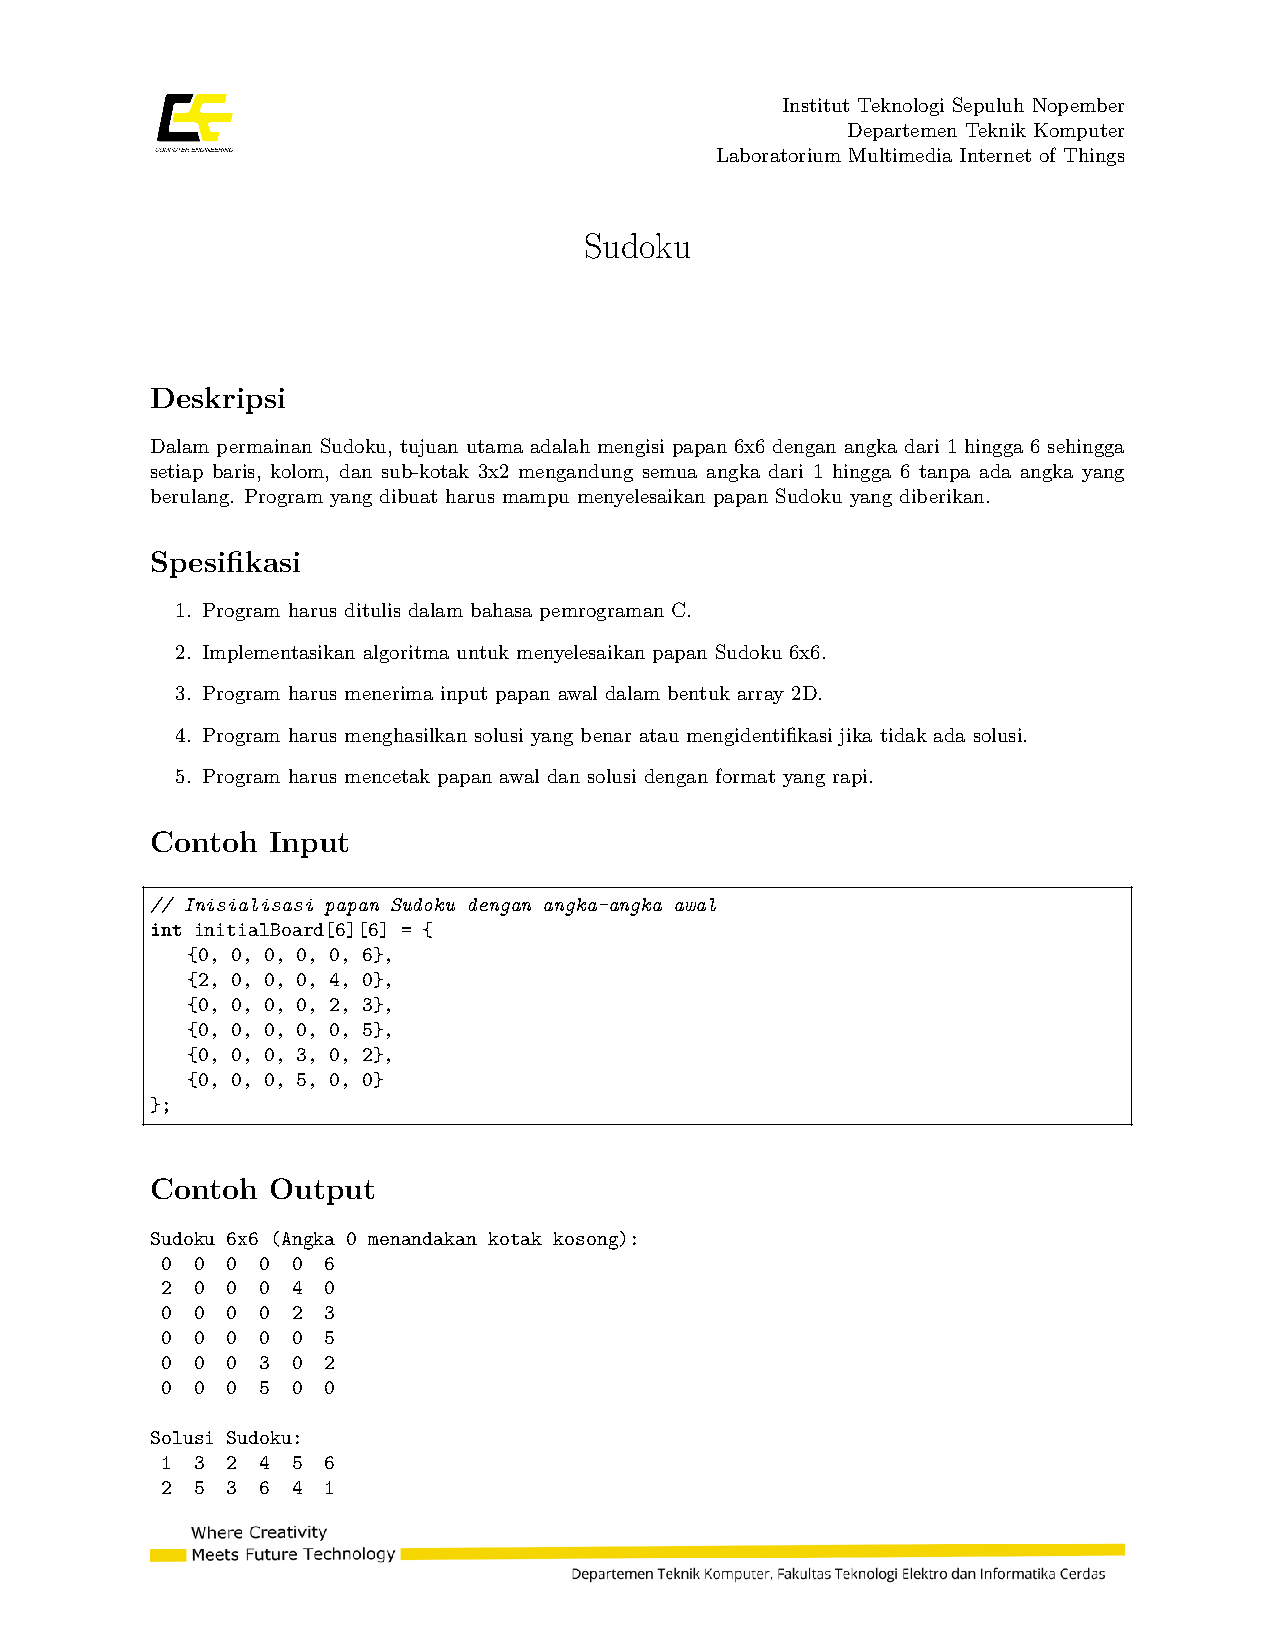
\includepdf[pages=-]{soal.pdf}
\setcounter{page}{1}

% Importing code from file
\section{Listing Kode}
\lstinputlisting[language=C]{main.c}
\clearpage

% di-ubah oleh Antonomasia, dari inisial F
\section{Lampiran Output}
\begin{lstlisting}[style=outputstyle]
  Microsoft Windows [Version 10.0.22635.2787]
  (c) Microsoft Corporation. All rights reserved.
  
  D:\Amiya\Documents\Dokumen\VSC\FP> cmd /C "c:\Users\Amiya\.vscode\extensions\ms-vscode.cpptools-1.18.5-win32-x64\debugAdapters\bin\WindowsDebugLauncher.exe --stdin=Microsoft-MIEngine-In-peoduojf.e5z --stdout=Microsoft-MIEngine-Out-b5qqg1dg.r1a --stderr=Microsoft-MIEngine-Error-blog4q2x.ibp --pid=Microsoft-MIEngine-Pid-4zlazad4.lbo "--dbgExe=C:\Program Files\CodeBlocks\MinGW\bin\gdb.exe" --interpreter=mi "
  Masukkan ukuran papan Sudoku: 6
  Masukkan papan Sudoku (gunakan 0 untuk kotak kosong):
  0 0 4 5 2 6
  0 0 0 1 0 3
  4 0 0 6 5 2
  2 5 6 3 0 0
  0 0 0 0 3 5
  5 4 3 2 6 1
  Papan awal Sudoku:
   0  0  4  5  2  6
   0  0  0  1  0  3
   4  0  0  6  5  2
   2  5  6  3  0  0
   0  0  0  0  3  5
   5  4  3  2  6  1
  
  Solusi Sudoku:
   3  1  4  5  2  6
   6  2  5  1  4  3
   4  3  1  6  5  2
   2  5  6  3  1  4
   1  6  2  4  3  5
   5  4  3  2  6  1
  
  D:\Amiya\Documents\Dokumen\VSC\FP>
\end{lstlisting}
\clearpage

% awikwok
\section{Deskripsi Program}
\par{Dalam permainan Sudoku, tujuan utama adalah mengisi papan 6x6 dengan angka dari 1 hingga 6 sehingga setiap baris, kolom, dan sub-kotak 3x2 mengandung semua angka dari 1 hingga 6 tanpa ada angka yang berulang. Program yang dibuat harus mampu menyelesaikan papan Sudoku yang diberikan.}
\par\null\par
\par{Spesifikasi dari program ini adalah ditulis dalam bahasa pemrograman C, implementasi algoritma untuk menyelesaikan papan Sudoku 6x6, menerima input papan awal dalam bentuk array 2D, menghasilkan solusi yang benar atau mengidentifikasi jika tidak ada solusi, dan mencetak papan awal dan solusi dengan format yang rapi. Program harus dapat dipahami dan diuji untuk memastikan hasilnya benar. Kode harus rapi dan mudah dibaca dengan komentar yang memadai.}
\par\null\par
\par{Tantangan Sudoku yang kompleks dapat diselesaikan dengan efektif dengan menggunakan pendekatan algoritma dan manajemen memori dinamis. Program ini, yang dibuat dalam bahasa pemrograman C, berfungsi untuk menerima input dari pengguna dalam bentuk papan Sudoku awal, menyelesaikan teka-teki, dan menemukan solusi atau tidak ada solusi. Dengan memungkinkan pengguna memasukkan ukuran papan yang mereka inginkan, program menjadi lebih fleksibel. Ini memungkinkan pengguna menangani Sudoku dalam berbagai ukuran.}
\par\null\par
\par{Memahami struktur program sangat penting untuk memahami cara menyelesaikan masalah Sudoku. Program ini terdiri dari beberapa fungsi utama yang berinteraksi satu sama lain. Pertama, fungsi "printSudoku" mencetak papan Sudoku ke layar menggunakan matriks NxN. Kemudian, fungsi "isValid" memverifikasi apakah angka dapat ditempatkan di baris dan kolom tertentu tanpa melanggar aturan Sudoku. Fungsi "solveSudoku", yang menggunakan algoritma backtracking dengan pendekatan rekursif, mencoba setiap kombinasi angka yang mungkin untuk mengisi papan, memeriksa validitasnya, dan mengulang prosedur hingga solusi ditemukan atau semua kemungkinan telah dijelajahi. inti dari program.}
\par\null\par
\par{Eksekusi program dimulai oleh fungsi "main". Setelah pengguna memasukkan ukuran papan Sudoku yang diinginkan (N), program mengalokasikan memori dinamis untuk matriks NxN. Kemudian, pengguna diminta untuk memasukkan elemen papan Sudoku sesuai dengan ukuran yang telah ditentukan. Untuk mencetak papan pertama Sudoku, program menggunakan fungsi "printSudoku" dan kemudian memanggil fungsi "solveSudoku" untuk menyelesaikan papan tersebut. Jika ditemukan solusi, solusi tersebut dicetak kembali ke layar dengan menggunakan "printSudoku", dan jika tidak ditemukan, program memberikan pemberitahuan bahwa tidak ada solusi yang valid. Terakhir, program menggunakan fungsi "free" untuk membebaskan memori yang telah dialokasikan untuk matriks Sudoku. Ini adalah langkah penting untuk mencegah kebocoran memori dan menjamin kinerja program yang baik.}
\par\null\par
\par{Alokasi memori dinamis adalah komponen penting dari program ini. Program dapat mengalokasikan memori sesuai dengan kebutuhan dengan meminta ukuran papan pengguna. Ini memberikan fleksibilitas dan memastikan penggunaan memori yang efisien. Deklarasi variabel pointer yang menunjuk ke baris matriks dilakukan pada awal proses. Program dapat mengalokasikan ruang memori untuk setiap baris dan kolom dalam matriks secara dinamis melalui fungsi "malloc". Ini membentuk struktur data dua dimensi yang dapat diakses secara efisien melalui indeks. Program menggunakan fungsi "free" untuk membebaskan memori yang telah dialokasikan setelah teka-teki diselesaikan dan solusi dicetak. Tindakan ini sangat penting untuk mencegah memori bocor dan memastikan program berjalan dengan lancar.}
\par\null\par
\par{Sangat penting untuk memahami bahwa algoritma backtracking adalah inti dari program ini untuk memecahkan Sudoku. Dengan fungsi rekursif "solveSudoku", aplikasi dapat dengan sistematis mempelajari setiap kombinasi angka yang mungkin. Program menggunakan rekursi untuk mencoba solusi lain sebelum kembali ke tingkat sebelumnya setelah menemukan solusi.}
\par\null\par
\par{Metode rekursif mempermudah menyelesaikan Sudoku yang lebih kompleks seiring dengan ukuran papan. Hal ini memungkinkan program untuk mencoba setiap kemungkinan dengan cepat dan efektif, dan hasil dicetak ke layar saat solusi ditemukan.}
\par\null\par
\par{Selain menawarkan solusi untuk permainan Sudoku, program ini juga berfungsi sebagai referensi bagi pengembang yang ingin mempelajari dan menggunakan konsep seperti alokasi memori dinamis, algoritma backtracking, dan manipulasi array dua dimensi dalam pemrograman C. Program ini memberikan gambaran yang jelas tentang bagaimana algoritma backtracking dapat digunakan untuk memecahkan teka-teki logika kompleks. Program ini menjadi lebih menarik karena dapat menangani Sudoku dalam berbagai ukuran berkat kemampuan untuk menyesuaikan ukuran papan dan manajemen memori dinamis. Karena algoritma backtracking yang tidak mampu memanfaatkan teknik pemecahan tingkat tinggi, program Sudoku yang ditulis dalam bahasa C memiliki kelemahan dalam menangani sudoku level expert, seperti "swordfish", "xy-wing", atau "hidden/naked subsets".}

\clearpage

\end{document}
